% Copyright 2026 Sreeram Anil
% SPDX-License-Identifier: CC-BY-4.0
% =============================================================================
%  Madgwick gradient-descent MARG filter — attitude (AHRS) family
% =============================================================================
\chapter{Gradient-Descent MARG Filter (Madgwick)}
\label{ch:att-madgwick}

\section*{At a glance}
\begin{tabular}{@{}l>{\raggedright\arraybackslash}p{0.76\textwidth}@{}}
Family & attitude / AHRS \\
Header & \texttt{include/estkit/attitude/madgwick.hpp} \\
Registered names & \texttt{Madgwick} (published), \texttt{Madgwick-Gated} (practical variant) \\
State & unit quaternion $\bm{q}\in S^3$ and gyro bias $\bm{b}\in\real^3$ (7 reals) \\
Cost per step & $\approx300$ flops, one \code{sqrt};
  $112$ / $\SI{138}{\nano\second}$ per step, 272\,bytes \\
Tuning & $\beta=0.1\,\SI{}{\radian\per\second}$, $\zeta=0$ (published defaults) \\
Primary references & \cite{madgwick2011,madgwick2010} \\
\end{tabular}

\section{Motivation and aerospace relevance}
Madgwick's filter is the cheapest MARG algorithm in wide use: no matrix, no covariance, one
normalisation and one tuning constant. It became the de-facto standard for small UAV autopilots,
motion capture and rehabilitation robotics precisely because it fits in a few hundred bytes on an
8-bit micro-controller and still fuses nine axes correctly.

Its conceptual contribution is to pose the vector-observation problem as an \emph{optimisation} and
then take exactly one normalised gradient step per sample. The gyro supplies the prediction; the
gradient step supplies a correction whose \emph{direction} is optimal in the least-squares sense and
whose \emph{magnitude} is a constant $\beta$. Choosing a constant magnitude rather than a
covariance-weighted one is what makes the filter cheap, and --- as this benchmark shows --- also
what makes it insensitive to the size of the disturbance it is fighting.

The second contribution is the magnetic-distortion compensation of
\cite[Sec.~3.3]{madgwick2010}: instead of a tabulated field vector, the reference is rebuilt each
step from the measurement itself, constrained to lie in the vertical plane containing magnetic
north. Any error in the assumed declination, and any horizontal distortion, is then confined to the
heading channel and cannot tilt the horizon. That trick is worth having in any MARG filter.

\section{Problem statement and assumptions}
Conventions as in Chapter~\ref{ch:att-complementary}: $\bm{q}$ maps BODY(FRD) to NAV(NED),
$\bm{R}(\bm{q})$ is its rotation matrix, the gyro measures $\bm{\omega}_y=\bm{\omega}+\bm{b}+\bm{n}_v$,
and the normalised specific force at rest equals $\bm{R}^\T\bm{d}_a$ with $\bm{d}_a=[0,0,-1]^\T$.

The filter assumes that the accelerometer measures gravity and that the magnetometer measures the
local field, with \emph{unknown but bounded} errors of total size $\omega_\beta$ expressed as an
equivalent gyro-rate error; $\beta=\sqrt{3/4}\,\omega_\beta$ is the resulting gain
\cite[Sec.~3.5]{madgwick2010}. It makes no distributional assumption and carries no uncertainty.

\subsection*{Frame mapping to this dataset}
Madgwick's published equations use a gravity reference $\bm{d}=[0,0,1]^\T$ together with an
accelerometer that reads $+1\,g$ on the vertical axis at rest (the ``reaction force'' convention in
a $z$-up earth frame). This benchmark is NED/FRD with the specific-force convention
$\bm{f}=\bm{a}-\bm{g}$, so a level accelerometer reads $[0,0,-g]^\T$ and the NAV reference of the
normalised accelerometer is
\begin{equation}
\bm{d}_a = [0,0,-1]^\T .
\label{eq:mw-da}
\end{equation}
Since the objective $\bm{f}_i$ and its Jacobian $\bm{J}_i$ defined below are both \emph{linear} in
$\bm{d}$, replacing $\bm{d}$ by $-\bm{d}$ changes the sign of both, and the gradient
$\bm{J}^\T\bm{f}$ is unchanged. This implementation is therefore bit-for-bit Madgwick's algorithm
applied to the negated accelerometer. The quaternion convention needs no change at all: Madgwick's
reference code propagates $\dot{\bm{q}}=\tfrac12\bm{q}\otimes[0,\bm{\omega}]$ with $\bm{\omega}$ in
the sensor frame and evaluates $\bm{R}(\bm{q})^\T\bm{d}$, which is exactly the BODY$\to$NAV Hamilton
quaternion used here. The magnetic part transfers verbatim because it uses the measured vertical
component whatever its sign (here $h_3>0$: the field dips downwards and NED $z$ points down).

\section{Derivation}

\subsection{The objective and its gradient}
Let $\bm{d}\in\real^3$ be a known NAV direction and $\bm{s}\in\real^3$ the corresponding measured
BODY direction, both unit. The orientation is correct when
\begin{equation}
\bm{f}(\bm{q};\bm{d},\bm{s}) \;=\; \bm{R}(\bm{q})^\T\bm{d}-\bm{s} \;=\; \bm{0}\in\real^3 ,
\label{eq:mw-f}
\end{equation}
an under-determined system (three equations, one unobservable rotation about $\bm{d}$) whose
least-squares solution is sought by steepest descent on
$F(\bm{q})=\tfrac12\norm{\bm{f}}^2$. With $\bm{q}=[q_w,q_x,q_y,q_z]$ the components of
\eqref{eq:mw-f} are
\begin{align}
f_1 &= d_1(1-2q_y^2-2q_z^2) + d_2(2q_xq_y+2q_wq_z) + d_3(2q_xq_z-2q_wq_y) - s_1,\nonumber\\
f_2 &= d_1(2q_xq_y-2q_wq_z) + d_2(1-2q_x^2-2q_z^2) + d_3(2q_yq_z+2q_wq_x) - s_2,\label{eq:mw-fexp}\\
f_3 &= d_1(2q_xq_z+2q_wq_y) + d_2(2q_yq_z-2q_wq_x) + d_3(1-2q_x^2-2q_y^2) - s_3,\nonumber
\end{align}
and the Jacobian $\bm{J}=\partial\bm{f}/\partial\bm{q}\in\real^{3\times4}$ is
\begin{equation}
\bm{J} = 2\!\begin{bmatrix}
 d_2q_z-d_3q_y & d_2q_y+d_3q_z & d_2q_x-d_3q_w-2d_1q_y & d_2q_w+d_3q_x-2d_1q_z\\
 d_3q_x-d_1q_z & d_1q_y+d_3q_w-2d_2q_x & d_1q_x+d_3q_z & d_3q_y-d_1q_w-2d_2q_z\\
 d_1q_y-d_2q_x & d_1q_z-d_2q_w-2d_3q_x & d_1q_w+d_2q_z-2d_3q_y & d_1q_x+d_2q_y
\end{bmatrix}.
\label{eq:mw-J}
\end{equation}
Substituting $\bm{d}=[0,0,1]^\T$ into \eqref{eq:mw-fexp}--\eqref{eq:mw-J} reproduces Madgwick's
Eqs.~(25)--(26) exactly; substituting \eqref{eq:mw-da} reproduces them with both signs flipped, as
argued above. With $m$ observations stacked,
\begin{equation}
\nabla F(\bm{q}) = \sum_{i=1}^{m}\bm{J}_i^\T\bm{f}_i \in\real^4,
\qquad
\dot{\bm{q}}_\varepsilon = \frac{\nabla F}{\norm{\nabla F}} .
\label{eq:mw-grad}
\end{equation}
The normalisation in \eqref{eq:mw-grad} is the crux of the method: the descent \emph{direction} is
computed from the data, the descent \emph{step} is the constant $\beta$. Madgwick's argument is
that the convergence rate of the estimate must merely exceed the divergence rate of the gyro
integration, and that the latter is bounded by $\omega_\beta$; a step proportional to the residual
would be faster when the residual is large, which is exactly when the residual is least likely to be
trustworthy.

\subsection{Fusion and the filter equations}
The two rates are combined and integrated with a single explicit Euler step:
\begin{align}
\dot{\bm{q}}_\omega &= \tfrac12\,\bm{q}\otimes[0,\bm{\omega}_c],\qquad \bm{\omega}_c=\bm{\omega}_y-\bm{b},\label{eq:mw-qw}\\
\dot{\bm{q}} &= \dot{\bm{q}}_\omega - \beta\,\dot{\bm{q}}_\varepsilon,\label{eq:mw-qdot}\\
\bm{q}_{k+1} &= \frac{\bm{q}_k+\dot{\bm{q}}\,\dt}{\norm{\bm{q}_k+\dot{\bm{q}}\,\dt}} .\label{eq:mw-int}
\end{align}
Equations \eqref{eq:mw-qw}--\eqref{eq:mw-int} are Madgwick's (42)--(44).

\subsection{Magnetic-distortion compensation (Sec.~3.3)}
Rather than a stored $\bm{m}_{\text{nav}}$, the reference is rebuilt each step from the measurement
by rotating it into the navigation frame and flattening its horizontal part onto north:
\begin{equation}
\bm{h} = \bm{R}(\bm{q})\,\hat{\bm{m}},\qquad
\bm{d}_m = \big[\sqrt{h_1^2+h_2^2},\;0,\;h_3\big]^\T .
\label{eq:mw-flux}
\end{equation}
By construction $\bm{d}_m$ has no east component, so the objective can never ask the filter to
change its \emph{inclination} estimate: an erroneous declination or a horizontal distortion is
absorbed entirely by the heading. The price is that the magnetometer no longer carries any
independent information about the dip angle, and therefore contributes less to roll and pitch than
a known reference would.

\subsection{Gyro-bias drift compensation (Sec.~3.4)}
The normalised gradient is a quaternion rate, so the body rate that would produce it is
\begin{equation}
\bm{\omega}_\varepsilon = 2\,\bm{q}^*\otimes\dot{\bm{q}}_\varepsilon
\quad(\text{vector part}),
\label{eq:mw-werr}
\end{equation}
which points along the axis about which the estimate is currently being corrected, i.e. along the
rate error that created the misalignment. Integrating it with gain $\zeta$ gives a bias estimate and
a corrected rate,
\begin{equation}
\bm{b}_{k+1}=\bm{b}_k+\zeta\,\bm{\omega}_\varepsilon\,\dt,
\qquad \bm{\omega}_c = \bm{\omega}_y-\bm{b} .
\label{eq:mw-bias}
\end{equation}
$\zeta$ has units of angular acceleration; Madgwick recommends $\zeta=\sqrt{3/4}\,\dot\omega_\beta$
with $\dot\omega_\beta$ the gyro bias drift rate. Because $\norm{\dot{\bm{q}}_\varepsilon}=1$ by
construction, $\norm{\bm{\omega}_\varepsilon}=2$ always: \eqref{eq:mw-bias} is a \emph{sign-like}
integrator that slews at a constant $2\zeta\,\SI{}{\radian\per\second\squared}$ regardless of how
large the bias error is. That makes it robust but also means it never settles --- it dithers about
the true bias with amplitude $2\zeta\dt$ per step.

\begin{remark}[Why $\zeta=0$ in the plain \texttt{Madgwick} instance]
The bias loop \eqref{eq:mw-bias} is driven by the same gradient that the manoeuvre disturbance
drives. On a fixed-wing mission with sustained coordinated turns, $\bm{\omega}_\varepsilon$ has a
long-lived non-zero mean during each turn, and the integrator walks: the measured bias RMSE on
\texttt{nominal} rises monotonically from $\SI{0.62}{\degree\per\second}$ (no estimate at all, i.e.
the true bias magnitude) at $\zeta=0$ to $1.00$, $1.50$ and $\SI{2.40}{\degree\per\second}$ at
$\zeta=0.005$, $0.01$ and $0.03$, and the attitude RMS rises with it. \emph{On its own}, $\zeta$ is
harmful; it is useful only together with disturbance rejection, which is why the two are enabled
together in the second registered instance (\S\ref{sec:mw-gated}) and neither is enabled in the
first. $\zeta=0$ also makes the plain instance identical to \code{ahrs.filters.Madgwick}: the
integrator's cross-validation measures a maximum angular difference of $0.0014^\circ$ over the
$9\times10^4$ samples of the nominal flight (Table~\ref{tab:val_ahrs}).
\end{remark}

\section{Algorithm}
\begin{algorithm}[H]
\caption{Madgwick MARG --- one sampling period}
\begin{algorithmic}[1]
\Require $\bm{q}_{k-1},\bm{b}_{k-1},\bm{\omega}_y,\bm{f},\bm{m}$; $\beta,\zeta$
\State $\hat{\bm{a}}\gets\bm{f}/\norm{\bm{f}}$, \; $\hat{\bm{m}}\gets\bm{m}/\norm{\bm{m}}$
\State $\nabla F \gets \bm{J}^\T(\bm{q},\bm{d}_a,\hat{\bm{a}})\,\bm{f}(\bm{q},\bm{d}_a,\hat{\bm{a}})$
       \Comment{$\bm{d}_a=[0,0,-1]^\T$, \eqref{eq:mw-da}}
\State $\bm{h}\gets\bm{R}(\bm{q})\hat{\bm{m}}$;\; $\bm{d}_m\gets[\sqrt{h_1^2+h_2^2},0,h_3]^\T$
       \Comment{flux compensation, \eqref{eq:mw-flux}}
\State $\nabla F \mathrel{+}= \bm{J}^\T(\bm{q},\bm{d}_m,\hat{\bm{m}})\,\bm{f}(\bm{q},\bm{d}_m,\hat{\bm{m}})$
\State $\dot{\bm{q}}_\varepsilon\gets\nabla F/\norm{\nabla F}$
\If{$\zeta>0$} \Comment{Sec.~3.4}
  \State $\bm{\omega}_\varepsilon\gets\operatorname{vec}(2\,\bm{q}^*\otimes\dot{\bm{q}}_\varepsilon)$;\;
         $\bm{b}\gets\operatorname{clamp}(\bm{b}+\zeta\bm{\omega}_\varepsilon\dt)$
\EndIf
\State $\dot{\bm{q}}\gets\tfrac12\bm{q}\otimes[0,\bm{\omega}_y-\bm{b}]-\beta\dot{\bm{q}}_\varepsilon$
\State $\bm{q}_k\gets(\bm{q}+\dot{\bm{q}}\dt)/\norm{\bm{q}+\dot{\bm{q}}\dt}$
\Ensure $\bm{q}_k,\bm{b}_k$
\end{algorithmic}
\end{algorithm}

\section{Application to the benchmark flight}
$\beta=0.1\,\SI{}{\radian\per\second}$ is the value the assignment prescribes and sits at the top of
Madgwick's recommended band: $\beta=\sqrt{3/4}\,\omega_\beta$ gives
$\omega_\beta=\SI{6.6}{\degree\per\second}$ of assumed gyro error, which is generous for the
$\SI{0.1}{\degree\per\second}$ noise and $\SI{0.5}{\degree\per\second}$ bias of the nominal
scenario. $\zeta=0$ and no manoeuvre gating: the \texttt{Madgwick} instance is the published algorithm,
nothing added. The \code{gate} switch in \code{Options} weights the two objectives in
\eqref{eq:mw-grad} by the disturbance weight \eqref{eq:cf-weight} of
Chapter~\ref{ch:att-complementary}; together with $\zeta=0.005$ it forms the second registered
instance, \texttt{Madgwick-Gated}, documented in \S\ref{sec:mw-gated}.

\section{Implementation notes}
The whole step is two evaluations of \eqref{eq:mw-fexp}--\eqref{eq:mw-J} (24 multiply--adds each
for $\bm{J}^\T\bm{f}$, plus about 40 for the entries), one 4-vector normalisation, one quaternion
product and one 4-vector normalisation: about 300 flops and a single \code{sqrt} beyond the two
measurement normalisations. Measured: $\SI{112}{\nano\second}$/step for the plain instance and
$\SI{138}{\nano\second}$ with the gate, the cheapest filter in the family that uses the gyro;
\code{sizeof} is 272\,bytes, of which $7\times8$ are the state. On a $\SI{216}{\mega\hertz}$
Cortex-M7 in float32 this is of order $\SI{2}{\micro\second}$/step, $0.02\,\%$ of the
$\SI{10}{\milli\second}$ budget at $\SI{100}{\hertz}$.

Guards: the accelerometer and magnetometer branches are skipped if the corresponding magnitude is
below $10^{-6}$; the gradient step is skipped if $\norm{\nabla F}<10^{-12}$, in which case the
filter degenerates gracefully to pure gyro integration; the quaternion is renormalised every step,
which is the only thing that keeps the explicit Euler integration \eqref{eq:mw-int} on the sphere;
the bias state is clamped to $\pm\SI{10}{\degree\per\second}$. The single-precision build reproduces
the double-precision mission RMS to five digits on \texttt{nominal}.

Two structural limitations are worth stating. First, \eqref{eq:mw-int} is an explicit Euler step:
the local truncation error is $O(\dt^2\norm{\ddot{\bm{q}}})$ and the renormalisation hides it, but at
low sample rates or high rates of turn it shows up as a lag. Second, there is no covariance, so the
filter cannot trade roll accuracy against heading accuracy, and it cannot tell a large residual
caused by a large attitude error from one caused by a large disturbance --- the correction is
$\beta$ either way.

\section{Benchmark results}
% Copyright 2026 Sreeram Anil
% SPDX-License-Identifier: CC-BY-4.0
\begin{table}[H]\centering\footnotesize\setlength{\tabcolsep}{3.5pt}\caption{Madgwick: attitude benchmark (mean over seeds; all angles in degrees; $t_\mathrm{conv}$: first time the attitude error stays below 2$^\circ$ for 30\,s; bias RMSE in deg/s; 272 bytes of state).}\label{tab:imu_Madgwick}
\begin{tabular}{lrrrrrrrrcr}\toprule scenario & RMS & roll & pitch & yaw & max & RMS$_\mathrm{ss}$ & $t_\mathrm{conv}$ [s] & bias RMSE & lost & ns/step \\ \midrule
nominal & 17.60 & 9.06 & 1.28 & 15.28 & 71.4 & 18.96 & -- & 1.03 & yes & 112 \\
init\_error & 17.74 & 9.14 & 1.73 & 15.37 & 71.4 & 18.96 & -- & 1.03 & yes & 112 \\
gyro\_bias & 17.62 & 9.01 & 1.29 & 15.33 & 69.4 & 19.41 & 281 & 3.80 & yes & 111 \\
mag\_disturbance & 19.01 & 9.06 & 1.48 & 16.87 & 71.4 & 18.96 & -- & 1.03 & yes & 109 \\
vibration & 14.78 & 8.40 & 1.76 & 12.27 & 50.9 & 16.53 & -- & 1.03 & yes & 112 \\
high\_dynamics & 18.43 & 9.41 & 1.42 & 16.04 & 81.8 & 19.58 & -- & 1.03 & yes & 111 \\
\bottomrule\end{tabular}\end{table}

\begin{figure}[H]\centering
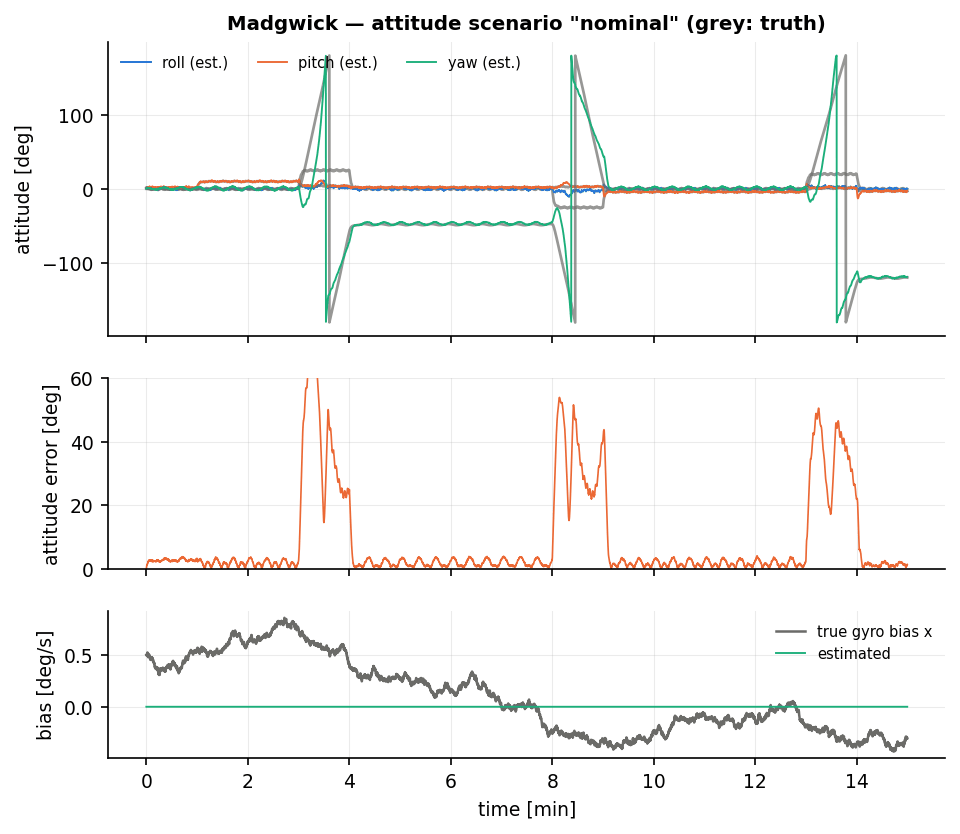
\includegraphics[width=\textwidth]{figures/imu_Madgwick_nominal.png}
\caption{Madgwick (published, $\beta=0.1$, $\zeta=0$) on the nominal mission: the three
$\SI{60}{\second}$ coordinated turns dominate the error budget.}
\end{figure}
\begin{figure}[H]\centering
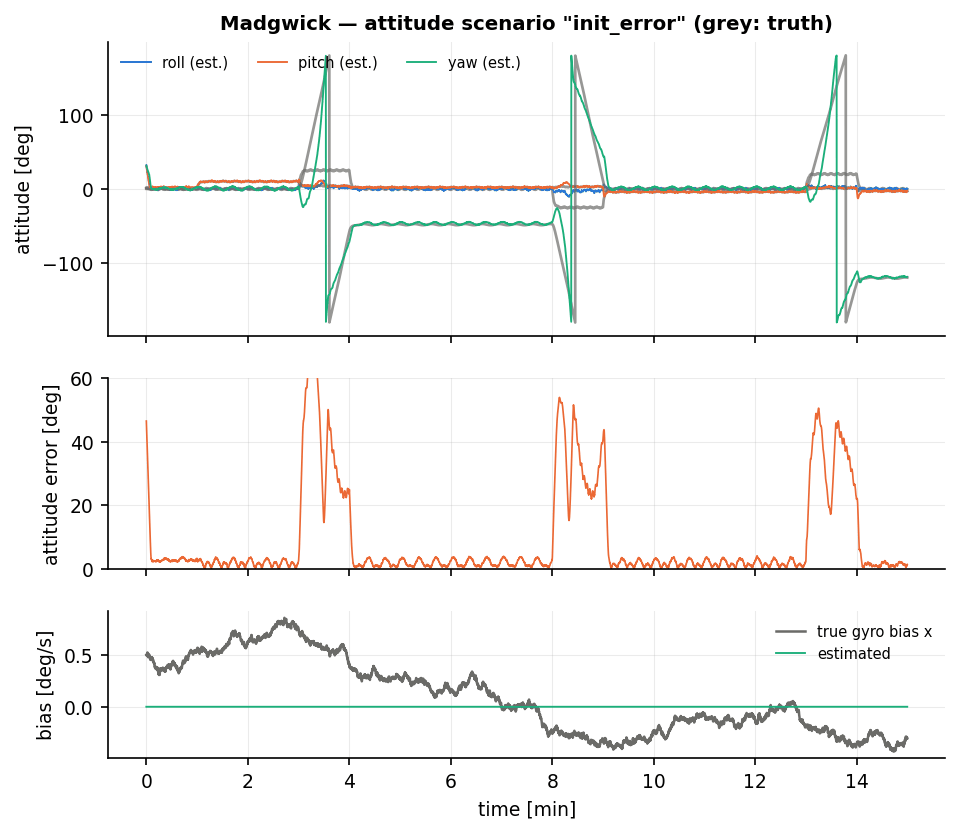
\includegraphics[width=\textwidth]{figures/imu_Madgwick_init_error.png}
\caption{Madgwick filter with a $46.6^\circ$ initial attitude error; the convergence rate is
limited by $\beta$, not by the size of the error.}
\end{figure}

On \texttt{nominal} the published filter gives $\text{RMS}=\SI{17.60}{\degree}$
(roll $9.06$, pitch $1.28$, yaw $\SI{15.28}{\degree}$), $\text{RMS}_{\text{ss}}=\SI{18.96}{\degree}$,
peak $\SI{71.4}{\degree}$, $\SI{112}{\nano\second}$/step, 272\,bytes, and is marked \emph{lost} on
every scenario but none. The per-phase breakdown (seed~1) explains the whole number at once:
\[
\underbrace{2.77}_{\text{take-off}}\;
\underbrace{2.07}_{\text{climb}}\;
\underbrace{\mathbf{42.05}}_{\text{turn 1}}\;
\underbrace{2.14}_{\text{cruise}}\;
\underbrace{\mathbf{35.52}}_{\text{turn 2}}\;
\underbrace{2.15}_{\text{descent}}\;
\underbrace{\mathbf{34.80}}_{\text{turn 3}}\;
\underbrace{1.53}_{\text{final}}\ \SI{}{\degree}.
\]
In level flight the filter is a $\SI{1.5}{\degree}$--$\SI{2.8}{\degree}$ device, i.e. within a
factor of two of the $\SI{0.65}{\degree}$ hard-iron floor of this dataset; during the three
$\SI{60}{\second}$ coordinated turns it is a $\SI{35}{\degree}$--$\SI{42}{\degree}$ device. The
mechanism is the one analysed in Chapter~\ref{ch:att-complementary}: in a coordinated turn the
accelerometer reports zero bank, and $\beta$ is a \emph{fixed} correction magnitude, so the filter
converges to the accelerometer's answer at the same rate whether that answer is right or wrong. The
$23^\circ$ tilt error is then amplified into $\approx\!50^\circ$ of heading error by the
$\tan I=2.14$ dip factor, which is why the yaw RMS ($15.28$) is larger than the roll RMS ($9.06$).

Table numbers are three-seed means; the sweeps below are single-seed (seed~1) diagnostics.

\paragraph{$\beta$ sensitivity.} On \texttt{nominal}:
$\beta=0.01\to13.95$, $0.033\to12.70$, $0.05\to15.41$, $0.1\to17.60$, $0.2\to18.68$,
$0.3\to\SI{18.99}{\degree}$. Smaller $\beta$ is better here for the obvious reason --- it slows the
filter's approach to the wrong accelerometer answer during the turns --- but it is not free:
$\beta=0.01$ costs $\SI{108.6}{\degree}$ on \texttt{gyro\_bias} (the correction can no longer keep
up with a $\SI{3}{\degree\per\second}$ drift, since $\beta$ must exceed the drift rate) and
$\SI{46.6}{\degree}$ on \texttt{vibration}. $\beta=0.033$ --- the bottom of the assignment's band ---
is the best compromise at $12.70/13.28/22.48/14.00/12.70/\SI{12.49}{\degree}$ across the six
scenarios, against $17.60/17.74/17.70/18.99/14.03/\SI{18.39}{\degree}$ for the registered
$\beta=0.1$. The registered value was kept because the assignment prescribes it and because
$\beta=0.1$ is the value most implementations ship.

\paragraph{$\zeta$ sensitivity.} At $\beta=0.1$ without gating,
\[
\zeta = 0\;/\;0.002\;/\;0.005\;/\;0.01\;/\;0.03
\ \Longrightarrow\
17.60\;/\;18.15\;/\;18.98\;/\;20.09\;/\;25.48\ \SI{}{\degree}
\]
with bias RMSE $0.62$, $0.63$, $1.00$, $1.50$ and $\SI{2.40}{\degree\per\second}$: the bias
integrator on its own is monotonically harmful, for the reason given in the remark above.

\paragraph{Other scenarios.} \texttt{vibration} is the only scenario on which the published filter
does \emph{better} than nominal ($14.78$ versus $\SI{17.60}{\degree}$): the added
$\SI{1}{\metre\per\second\squared}$ of broadband accelerometer noise perturbs the gradient
\emph{direction} but not its magnitude, and the constant-$\beta$ step averages it out --- an
accidental benefit of not being covariance-weighted. \texttt{mag\_disturbance} costs
$\SI{1.4}{\degree}$ ($19.01$); the flux compensation \eqref{eq:mw-flux} confines the
$\SI{25}{\micro\tesla}$ offset to the heading, as designed. \texttt{gyro\_bias} costs almost nothing
($17.62$) because $\beta\gg$ the bias: the correction bandwidth is set by $\beta$, not by the
disturbance --- and, oddly, it is the only scenario on which the plain filter passes the convergence
test ($t_{\text{conv}}=\SI{281}{\second}$), because a large bias briefly biases the estimate
\emph{towards} truth during one of the turns. Turning the magnetometer off
(\code{use\_mag=false}) gives $\SI{87.4}{\degree}$, confirming that heading is unobservable from
gravity alone.

\paragraph{Initial-error transient.} Starting from $46.6^\circ$ of attitude error the filter needs
$\SI{5.3}{\second}$ to reach $5^\circ$; from $78.5^\circ$, $\SI{9.5}{\second}$; from $90^\circ$,
$\SI{10.3}{\second}$. The slope is $\approx\SI{7.9}{\degree\per\second}$ and is independent of the
error, as \eqref{eq:mw-qdot} requires (the body-rate magnitude of the correction is at most
$2\beta=\SI{11.5}{\degree\per\second}$). Compare the MEKF's $\SI{0.17}{\second}$ and the invariant
EKF's $\SI{0.01}{\second}$ from the same $46.6^\circ$: a covariance-weighted filter knows that the
residual is large because the \emph{state} is wrong, and takes a correspondingly large step.

\section{The gated variant (\texttt{Madgwick-Gated})}\label{sec:mw-gated}
The second registered instance switches on both of the mechanisms that the published algorithm
leaves out, and it is important to be explicit that this is an \textbf{engineering addition, not
part of Madgwick's method}: the objectives in \eqref{eq:mw-grad} are weighted by the disturbance
weight \eqref{eq:cf-weight} of Chapter~\ref{ch:att-complementary} (magnitude anomaly plus the
rate-driven manoeuvre bound of Chapter~\ref{ch:att-mekf}, Remark~\ref{rem:mekf-turn}), and the
bias-drift compensation of Sec.~3.4 is enabled with $\zeta=0.005$. Everything else --- $\beta=0.1$,
the gradient \eqref{eq:mw-grad}, the flux compensation \eqref{eq:mw-flux}, the explicit Euler step
\eqref{eq:mw-int} --- is unchanged, and the cost rises only from $112$ to
$\SI{138}{\nano\second}$/step at the same 272\,bytes.

\begin{remark}[The gate and the bias state are a package deal]\label{rem:mw-package}
The manoeuvre detector needs an angular rate that is free of bias, because it declares a manoeuvre
whenever $V_{\text{ref}}\norm{\bm{\omega}_{yz}}$ exceeds a threshold. With $\zeta=0$ there is no
bias estimate, so on \texttt{gyro\_bias} the $\SI{3}{\degree\per\second}$ offset looks like a
permanent turn, the accelerometer is latched off for the whole mission, and only the magnetometer
remains: measured $\SI{55.3}{\degree}$ RMS, against $\SI{10.1}{\degree}$ on nominal. Conversely
$\zeta>0$ without the gate walks, as shown above. Enabling both gives
$\SI{4.81}{\degree}$ on \texttt{nominal} and $\SI{4.81}{\degree}$ on \texttt{gyro\_bias} (seed~1) ---
the two mechanisms fix each other's failure mode, and either one alone is worse than neither.
\end{remark}

% Copyright 2026 Sreeram Anil
% SPDX-License-Identifier: CC-BY-4.0
\begin{table}[H]\centering\footnotesize\setlength{\tabcolsep}{3.5pt}\caption{Madgwick-Gated: attitude benchmark (mean over seeds; all angles in degrees; $t_\mathrm{conv}$: first time the attitude error stays below 2$^\circ$ for 30\,s; bias RMSE in deg/s; 272 bytes of state).}\label{tab:imu_MadgwickGated}
\begin{tabular}{lrrrrrrrrcr}\toprule scenario & RMS & roll & pitch & yaw & max & RMS$_\mathrm{ss}$ & $t_\mathrm{conv}$ [s] & bias RMSE & lost & ns/step \\ \midrule
nominal & 5.78 & 2.48 & 2.46 & 4.60 & 22.8 & 7.43 & -- & 0.22 & no & 138 \\
init\_error & 6.17 & 2.75 & 2.72 & 4.88 & 46.5 & 7.43 & -- & 0.30 & no & 140 \\
gyro\_bias & 5.79 & 2.48 & 2.46 & 4.60 & 22.8 & 7.43 & -- & 0.44 & no & 138 \\
mag\_disturbance & 5.78 & 2.48 & 2.46 & 4.59 & 22.8 & 7.43 & -- & 0.22 & no & 136 \\
vibration & 3.22 & 1.67 & 1.78 & 2.08 & 12.5 & 3.52 & 263 & 0.17 & no & 138 \\
high\_dynamics & 5.34 & 2.78 & 2.58 & 3.76 & 16.6 & 6.20 & -- & 0.24 & no & 129 \\
\bottomrule\end{tabular}\end{table}

\begin{figure}[H]\centering
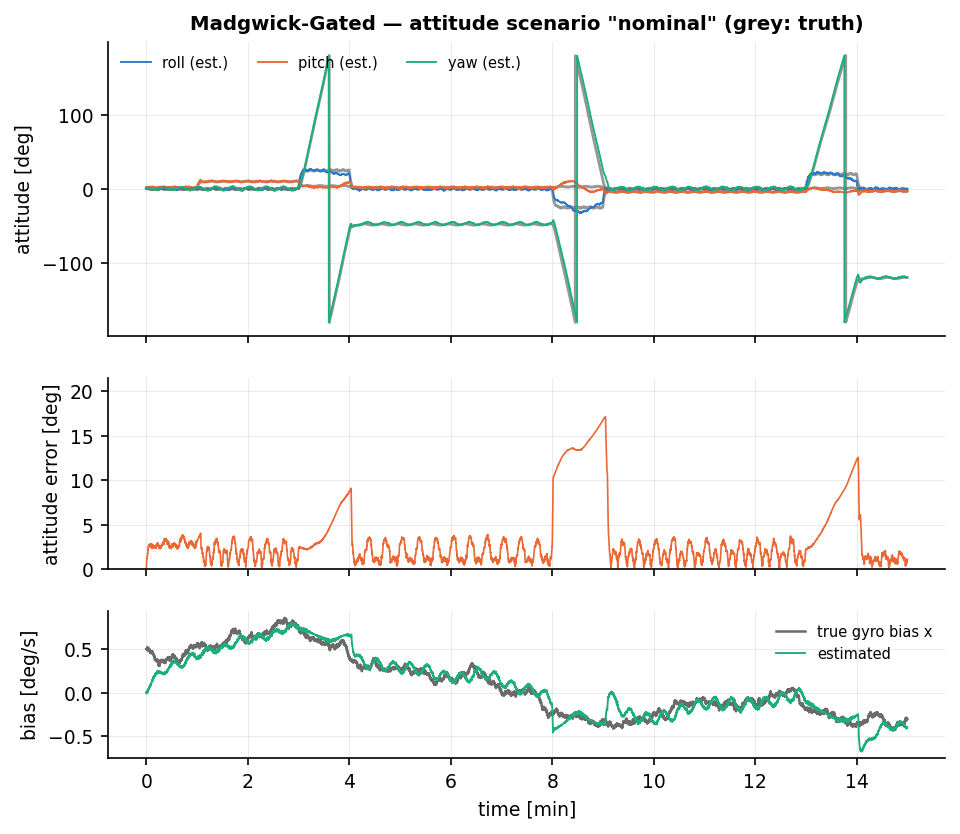
\includegraphics[width=\textwidth]{figures/imu_MadgwickGated_nominal.png}
\caption{Madgwick-Gated on the nominal mission: with the manoeuvre gate the three coordinated turns
are reduced from $\approx40^\circ$ to $5$--$\SI{14}{\degree}$ of error.}
\end{figure}

\texttt{Madgwick-Gated} gives $5.78/6.17/5.79/5.78/3.22/\SI{5.34}{\degree}$ across the six scenarios
in table order, a factor of three better than the published instance, with bias RMSE
$\SI{0.22}{\degree\per\second}$ (against the true $\SI{1.03}{\degree\per\second}$), peak error
$\SI{22.8}{\degree}$ instead of $71.4$, and \emph{no} lost-track flag anywhere. Per phase (seed~1)
\[
2.78\;/\;2.13\;/\;5.08\;/\;2.04\;/\;13.86\;/\;2.08\;/\;7.36\;/\;1.33\ \SI{}{\degree},
\]
so the turns fall from $42/36/\SI{35}{\degree}$ to $5.1/13.9/\SI{7.4}{\degree}$ while the level
phases are unchanged --- the gate does exactly what it is designed to do and nothing else. It is
also the best \texttt{vibration} result of any filter outside the Kalman pair
($\SI{3.22}{\degree}$, $t_{\text{conv}}=\SI{263}{\second}$), because the low-passed magnitude test
correctly declines to treat zero-mean vibration as a manoeuvre.

Two honest caveats. First, the gated filter still does not pass the $2^\circ$ convergence test on
\texttt{nominal}: its floor is $\SI{5.8}{\degree}$, an order of magnitude above the
$\SI{0.65}{\degree}$ sensor floor, because $\beta$ remains a fixed step size and cannot exploit the
much better accelerometer that the gate has now handed it. Compare \texttt{Mahony-Gated}
(Chapter~\ref{ch:att-mahony}), which applies the same gate to a filter whose gain \emph{is}
proportional to the residual and reaches $\SI{2.14}{\degree}$ at the same cost. Second, the
large-initial-error transient is unchanged and still $\beta$-limited: $\SI{5.2}{\second}$ to
$5^\circ$ from $46.6^\circ$, $\SI{13.4}{\second}$ from $78.5^\circ$. The gate buys disturbance
rejection, not bandwidth.

\section{Summary}
Madgwick's filter is the best flops-per-degree bargain in the family in level flight: 272\,bytes,
$\SI{112}{\nano\second}$/step, and $\SI{1.5}{\degree}$--$\SI{2.8}{\degree}$ of error on every phase
that is not a sustained turn. Use it on hand-held, ground or rotary-wing platforms whose specific
force is gravity most of the time. Do not use it on a fixed-wing aircraft without adding manoeuvre
rejection: the constant step size $\beta$ that makes it robust also makes it converge to a wrong
accelerometer at full speed, and the three coordinated turns of this mission cost it a factor of
seven in mission RMS ($17.60$ versus $\SI{2.48}{\degree}$ for the MEKF). If manoeuvre rejection is
added, switch $\zeta$ on with it --- Remark~\ref{rem:mw-package}: the two are worse than useless
apart and give $\SI{5.78}{\degree}$ together, at $\SI{138}{\nano\second}$/step. Neither addition is
Madgwick's; both are ours.
